
\section{Spray : un protocole d'échantillonnage adaptatif}

\SPRAY est un protocole d'échantillonnage de paris adaptatif inspiré à la fois
de \SCAMP~\cite{ganesh2003peer} et \CYCLON~\cite{voulgaris2005cyclon}. \SPRAY
comprend trois parties représentant le cycle de vie d'un pair dans le
réseau. Tout d'abord, le processus consistant à rejoindre le réseau, qui injecte
un nombre logarithmique d'arcs comparé à la taille du réseau. De ce fait, le
nombre d'arcs passe à l'échelle. Ensuite, chaque pair éxecute un processus
periodique dont le but est d'équilibrer les vues partielles en termes de taille
et d'uniformité sur les pairs références dans celles-ci. Le réseau converge
rapidement vers une topologie possédant des propriétés similaires à celles des
graphes aléatoires. Enfin, un pair est capable de quitter le réseau à n'importe
quel moment sans en notifier le réseau (l'équivalent d'un crash) sans dégrader
les propriétés du reste du réseau.

L'obtention de cette propriété d'adaptivité repose essentiellement sur le fait
de conserver un nombre d'arcs cohérent durant tout le cycle de vie du réseau.
En effet, en opposition à \CYCLON, \SPRAY est toujours à la limite du nombre
optimal d'arcs. Comme \SPRAY n'ajoute jamais d'arcs après le processus d'entrée,
toute suppression d'arcs est définitive et ne doit donc pas être pris à la
légère. Ainsi, \SPRAY ajoute des arcs dans un premier temps. Dans un second
temps, le processus periodique de mélange des arcs de \SPRAY préserve tous les
arcs du réseau.  Dans un troisième temps, le processus de sortie supprime
précautionneusement quelques arcs. Dans l'idéal, il s'agit du nombre d'arcs
ajouté par le dernier pair entré dans le réseau.

Parfois, conserver le nombre d'arcs global constant force les processus de
mélange et de sortie à créer des doublons dans les vues partielles. Ainsi, une
vue partielle peut contenir plusieurs fois le même voisin. Toutefois, ces
doublons restent peu nombreux, et de ce fait, n'ont pas d'impact notable sur la
connectivité du réseau.

\subsection{Rejoindre le réseau}

L'algorithme pour rejoindre le réseau est, dans \SPRAY, la seule manière
d'introduire de nouveaux arcs dans le réseau. Afin de répondre à la première
partie de l'énoncé du problème (REF), ce nombre d'arcs doit augmenter
logarithmiquement comparé à la taille du réseau. Tout comme dans \SCAMP, nous
supposons que chacuns des pairs respecte cette contrainte. Dès lors, ces
derniers utilisent ce savoir afin de propager l'identité du nouvel
arrivant. L'algorithme~\ref{algo:joining} décrit la façon dont le contact envoie
la nouvelle identité à son voisinage où elle est intégrée directement à leur vue
partielle. En définitive, le nombre d'arcs dans le réseau augmente de
$1+\ln(|\mathcal{N}|)$ et ce, seulement en utilisant des interactions de voisin
à voisin.

\begin{figure*}
  \centering
  \subfloat[Figure A][$p_1$ contacts $p_2$ to join the network. $p_1$ adds
  $p_2$ to its neighborhood. $p_1$ sends its request to $p_2$.]{
    
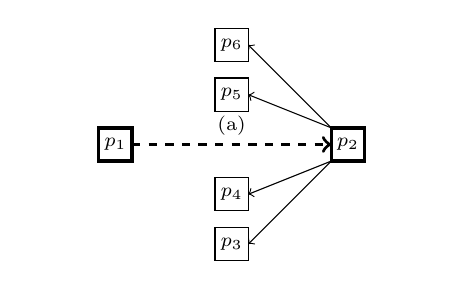
\begin{tikzpicture}[scale=1.2]

  \newcommand\X{35pt};
  \newcommand\Y{15pt};

  \draw(-0.75*\X, 0pt); %% positioning
  \draw( 2.75*\X, 0pt); %% positioning

  \scriptsize
  \draw[->,dashed,very thick](5+0*\X, 0*\Y) -- 
  node[anchor=south]{(a)}(-5+ 2*\X, 0*\Y);
  \draw[->] (-5+2*\X, 5pt) -- (5+\X, \Y);
  \draw[->] (-5+2*\X, 5pt) --  (5+\X, 2*\Y);
  \draw[->] (-5+2*\X, -5pt) -- (5+\X, -\Y);
  \draw[->] (-5+2*\X, -5pt) -- (5+\X, -2*\Y);

  \draw[fill=white, very thick]
  (0*\X, 0*\Y) node{$p_1$} +(-5pt,-5pt) rectangle +(5pt,5pt);
  \draw[fill=white, very thick]
  (2*\X, 0*\Y) node{$p_2$} +(-5pt,-5pt) rectangle +(5pt,5pt);

  \draw[fill=white](1*\X,2*\Y) node{$p_6$} +(-5pt,-5pt) rectangle +(5pt,5pt);
  \draw[fill=white](1*\X,1*\Y) node{$p_5$} +(-5pt,-5pt) rectangle +(5pt,5pt);
  \draw[fill=white](1*\X,-1*\Y) node{$p_4$} +(-5pt,-5pt) rectangle +(5pt,5pt);
  \draw[fill=white](1*\X,-2*\Y) node{$p_3$} +(-5pt,-5pt) rectangle +(5pt,5pt);
  
\end{tikzpicture}}
  \hspace{8pt}
  \subfloat[Figure B][The $onSubs(p_1)$ event is raised at $p_1$
  which forwards the subscription to $p_1$'s neighborhood.]{
    
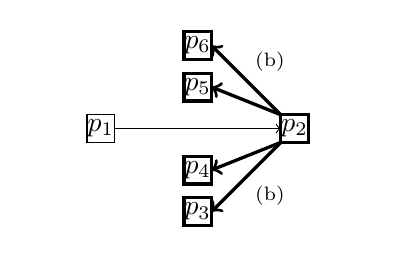
\begin{tikzpicture}[scale=1]

  \newcommand\X{35pt};
  \newcommand\Y{15pt};

  \draw(-0.75*\X, 0pt); %% positioning
  \draw( 2.75*\X, 0pt); %% positioning

  \scriptsize
  \draw[->](5+0*\X, 0*\Y) -- (-5+ 2*\X, 0*\Y);
  \draw[->, very thick] (-5+2*\X, 5pt) -- (5+\X, \Y);
  \draw[->, very thick] (-5+2*\X, 5pt) --
  node[anchor=south west]{(b)} (5+\X, 2*\Y);
  \draw[->, very thick] (-5+2*\X, -5pt) -- (5+\X, -\Y);
  \draw[->, very thick] (-5+2*\X, -5pt) --
  node[anchor=north west]{(b)}(5+\X, -2*\Y);

  \normalsize
  \draw[fill=white]
  (0*\X, 0*\Y) node{$p_1$} +(-5pt,-5pt) rectangle +(5pt,5pt);
  \draw[fill=white, very thick]
  (2*\X, 0*\Y) node{$p_2$} +(-5pt,-5pt) rectangle +(5pt,5pt);

  \draw[fill=white, very thick]
  (1*\X,2*\Y) node{$p_6$} +(-5pt,-5pt) rectangle +(5pt,5pt);
  \draw[fill=white, very thick]
  (1*\X,1*\Y) node{$p_5$} +(-5pt,-5pt) rectangle +(5pt,5pt);
  \draw[fill=white, very thick]
  (1*\X,-1*\Y) node{$p_4$} +(-5pt,-5pt) rectangle +(5pt,5pt);
  \draw[fill=white, very thick]
  (1*\X,-2*\Y) node{$p_3$} +(-5pt,-5pt) rectangle +(5pt,5pt);

\end{tikzpicture}}
  \hspace{8pt}
  \subfloat[Figure C][The $onFwdSubs(p_1)$ event is raised at $p_{3-6}$. The
  peers add $p_1$ to their neighborhood.]{
    
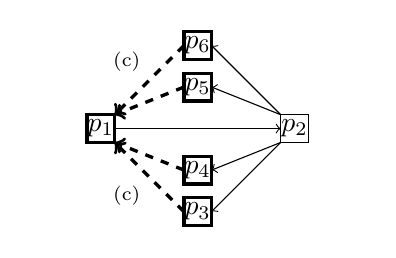
\begin{tikzpicture}[scale=1]

  \newcommand\X{35pt};
  \newcommand\Y{15pt};

  \draw(-0.75*\X, 0pt); %% positioning
  \draw( 2.75*\X, 0pt); %% positioning

  \scriptsize
  \draw[->](5+0*\X, 0*\Y) -- (-5+ 2*\X, 0*\Y);
  \draw[->] (-5+2*\X, 5pt) -- (5+\X, \Y);
  \draw[->] (-5+2*\X, 5pt) -- (5+\X, 2*\Y);
  \draw[->] (-5+2*\X, -5pt) -- (5+\X, -\Y);
  \draw[->] (-5+2*\X, -5pt) -- (5+\X, -2*\Y);

  \draw[->,dashed, very thick](-5+\X, 2*\Y) --
  node[anchor=south east]{(c)} ( 5pt,5pt);
  \draw[->,dashed, very thick](-5+\X, 1*\Y) -- ( 5pt,5pt);
  \draw[->,dashed, very thick](-5+\X, -1*\Y) -- ( 5pt,-5pt);
  \draw[->,dashed, very thick](-5+\X, -2*\Y) --
  node[anchor=north east]{(c)}( 5pt,-5pt);

  \normalsize
  \draw[fill=white, very thick]
  (0*\X, 0*\Y) node{$p_1$} +(-5pt,-5pt) rectangle +(5pt,5pt);
  \draw[fill=white]
  (2*\X, 0*\Y) node{$p_2$} +(-5pt,-5pt) rectangle +(5pt,5pt);

  \draw[fill=white, very thick]
  (1*\X,2*\Y) node{$p_6$} +(-5pt,-5pt) rectangle +(5pt,5pt);
  \draw[fill=white, very thick]
  (1*\X,1*\Y) node{$p_5$} +(-5pt,-5pt) rectangle +(5pt,5pt);
  \draw[fill=white, very thick]
  (1*\X,-1*\Y) node{$p_4$} +(-5pt,-5pt) rectangle +(5pt,5pt);
  \draw[fill=white, very thick]
  (1*\X,-2*\Y) node{$p_3$} +(-5pt,-5pt) rectangle +(5pt,5pt);
 

\end{tikzpicture}}
  \caption{\label{fig:joiningexample}Example of the \SPRAY's joining
    protocol.}
\end{figure*}

\begin{algorithm}

\small
\algrenewcommand{\algorithmiccomment}[1]{\hskip2em$\rhd$ #1}

\newcommand{\comment}[1]{$\rhd$ #1}


\algblockdefx[initially]{initially}{endInitially}
  [0] {\textbf{INITIALLY:}} 

\algblockdefx[pas]{pas}{endPas}
  [0] {\textbf{EVENTS:}}

\newcommand{\LINEFOR}[2]{%
  \algorithmicfor\ {#1}\ \algorithmicdo\ {#2} %
  }

\newcommand{\LINEIFTHEN}[2]{%
  \algorithmicif\ {#1}\ \algorithmicthen\ {#2} %
  }

\newcommand{\INDSTATE}[1][1]{\State\hspace{\algorithmicindent}}

\begin{algorithmic}[1]
  \Statex
  \initially
    \State $\mathcal{P} \leftarrow \varnothing$;
    \hfill \comment{the partial view is a multiset}
    \State $p$ ; \hfill \comment{identity of the local peer}
  \endInitially
  
  \pas
  \Function{onSubs}{$o$} \hfill \comment{$o: origin$}
    \State \LINEFOR{\textbf{each} $\langle q,\,\_\, \rangle \in\mathcal{P}$}
    {$sendTo(q,\, 'fwdSubs',\, o)$;} \label{line:multicast}
    \EndFunction
    \Statex
    \Function{onFwdSubs}{$o$} \hfill \comment{$o: origin$}
    \State $\mathcal{P} \leftarrow
    \mathcal{P}\uplus \left\{\langle o,\, 0 \rangle\right\}$;
    \EndFunction
  \endPas
  
\end{algorithmic}

\caption{\label{algo:joining}The joining protocol of \SPRAY.}
\end{algorithm}

La vue partielle est un multiensemble de couples $\langle n,\, age\rangle$ qui
associe à chaque voisin $n$ l'âge $age$. Ce multiensemble permet de gérer les
doublons. L'âge joue le même rôle que dans \CYCLON, çàd qu'il accélère la
suppression des pairs qui sont sortis ou ont crash. L'évenement $onSubs$ est
appelé chaque fois qu'un pair rejoins le réseau via ce contact. $onSubs$
redirige l'identité du pairs à tous ses voisins, indépendament de
l'âge. L'évenement $onFwdSubs$ est déclanché lorsqu'un pair reçoit une telle
identité redirigée. $onFwdSubs$ ajoute la référence en initialisant son âge à
$0$.

La figure~\ref{fig:joiningexample} décrit un scenario où le pair $p_1$ contacte
le pair $p_2$ afin de rejoindre le réseau composé de $\{p_2$, $p_2$, $p_4$,
$p_5$, $p_6\}$. Pour simplifier, la figure ne montre que les arcs nouvellement
introduit ainsi que le voisinage de $p_1$ et $p_2$. Le pair $p_1$ ajoute
directement $p_2$ dans sa vue partielle. Ce dernier redirige l'identité de $p_1$
à chacun de ses voisins.  Chacun de ces voisins ajoute alors $p_1$ à leur vue
partielle. Au total, \SPRAY établie 5 connexions. Le réseau en résultant est
connecté.

Malheureusement, les vues partiels des derniers arrivant sont clairement
déséquilibrés comparé au reste du réseau. De ce fait, ils violent la première
condition de l'énoncé du problème (REF). Le processus de mélange décrit dans la
prochaine section a pour but de ré-équilibrer les vues partielles.

\subsection{Échanger son voisinage}

Au contraire de \CYCLON, \SPRAY mélange des vues partielles dont les tailles
peuvent être différentes. Ce processus à pour but d'équilibrer les tailles de
vue partielles ainsi que de mélanger les références à l'interieur de celles-ci.
Ce processus à pour contrainte de conserver l'exact même nombre d'arcs.

Les deux pairs impliqués dans le mélange s'envoient l'un l'autre la moitié de
leur vue partielle. Après l'intégration de ces nouvelles références, la taille
de leur vue partielle tend vers la moyenne, et la somme globale en demeure
inchangée. Dans ce but, les vues partielles sont des multiensembles. Ainsi, si
un pair réçoit une référence déjà connue, il la conserve en tant que doublon.
De cette façon, le nombre d'arcs reste constant.

Si les doublons ont un impact négatif sur les propriétés du réseau, la plupart
de ceux-ci disparaissent après le processus de mélange. En proportion, ils
deviennent négligeable dès lors que le réseau grandit.

\begin{algorithm}[h]
  
\small
\algrenewcommand{\algorithmiccomment}[1]{\hskip2em$\rhd$ #1}

\newcommand{\comment}[1]{$\rhd$ #1}

\algblockdefx[act]{act}{endAct}
  [0] {\textbf{ACTIVE THREAD:}}

\algblockdefx[pas]{pas}{endPas}
  [0] {\textbf{PASSIVE THREAD:}}


\newcommand{\LINEFOR}[2]{%
  \algorithmicfor\ {#1}\ \algorithmicdo\ {#2} %
  }

\newcommand{\LINEIFTHEN}[2]{%
  \algorithmicif\ {#1}\ \algorithmicthen\ {#2} %
  }

\newcommand{\INDSTATE}[1][1]{\State\hspace{\algorithmicindent}}

\begin{algorithmic}[1]
  \Statex
  \act
    \Function{loop}{ } \hfill \comment{Every $\Delta\,t$}
    \State $\mathcal{P} \leftarrow incrementAge(\mathcal{P})$;
    \State \textbf{let} $ \langle q,\, age \rangle \leftarrow getOldest(\mathcal{P})$;
    \State \textbf{let} $sample \leftarrow $ \label{line:samplesize}
    $getSample(\mathcal{P}\setminus\left\{\langle q, age\rangle\right\}, \left \lceil{|\mathcal{P}|\over{2}} \right \rceil-1) \uplus \left\{\langle p, 0 \rangle\right\}$;
    \State $sample \leftarrow replace(sample,\,q,\,p)$; \label{line:replace1}
    \State $sendTo(q,\, 'exchange',\, sample)$;
    \State \textbf{let} $sample'\leftarrow receiveFrom(q)$;
    \State $sample \leftarrow replace(sample,\,p,\,q)$;
    \State $\mathcal{P} \leftarrow (\mathcal{P} \setminus sample) \uplus
    sample'$;
    \EndFunction
  \endAct
  
  \pas
    \Function{onExchange}{$o,\, sample$} \hfill \comment{$o: origin$}
    \State \textbf{let} $sample' \leftarrow getSample(\mathcal{P} ,\, \left\lceil |\mathcal{P}|\over{2} \right\rceil )$;
    \State $sample' \leftarrow replace(sample',\,o,\,p);$ \label{line:replace2}
    \State $sendTo(o ,\, sample')$;
    \State $sample' \leftarrow replace(sample',\,p,\,o)$;
    \State $\mathcal{P} \leftarrow (\mathcal{P} \setminus sample') \uplus
    sample$; 
    \EndFunction
  \endPas
  
\end{algorithmic}

  \caption{\label{algo:scamplon}The cyclic protocol of \SPRAY.}
\end{algorithm}

L'algorithme~\ref{algo:scamplon} montre la partie periodic de \SPRAY éxécutée
par chaque pair. Il est divisé en deux parties, à savoir le processus actif qui
est appelé régulièrement afin d'initier un mélange de vues, et le processus
passif qui réagit au message du processus actif. Les fonctions qui ne sont pas
explicitement définies sont les suivantes:
\begin{compactitem}
\item $incrementAge(view)$ : incrémente l'âge des éléments présent dans la vue
  $view$ et retourne la vue modifiée.
\item $getOldest(view)$ : retourne le plus vieu des pairs présent dans la vue.
\item $getSample(view,\, size)$ : retourne un échantillon de la vue contenant $size$
  éléments.
\item $replace(view,\,old,\,new)$ : remplace les occurrences de $old$ par $new$ dans
  la vue $view$.
\item $rand()$ : retourne un nombre flottant aléatoire entre $0$ et $1$.
\end{compactitem}

Dans le processus actif, la fonction $loop$ est appelée tous les intervals
$\Delta$ de temps. Tout d'abord, la fonction incrémente l'age de chacun des
voisins dans la vue partielle $\mathcal{P}$. Ensuite, le pair le plus âgé $q$
est choisit afin d'initier un échange. Si le pair $q$ ne peut être joint (car il
est parti ou a crash), alors le pair $p$ éxecute la fonction qui gère ce cas
(voir la section suivante). 

\subsection{Quitter le réseau}

%%% Local Variables:
%%% mode: latex
%%% TeX-master: "../../paper"
%%% End:
